\section{Development Model}
\label{sec:development}

To satisfy the mission statement of the Project, the SunPy community adopted an open development model.
This development model is widely used within the scientific Python community.
The \sunpypkg package is hosted on \github and uses Git\footnote{\url{https://git-scm.com/}} as its distributed version control software.
The entire codebase is publicly available and anyone can suggest changes through pull requests.
Since the codebase is licensed under a permissive 2-clause BSD license\footnote{\url{https://opensource.org/licenses/BSD-2-Clause}}, anyone can redistribute, improve, repackage or use it in a closed environment as long as they credit the SunPy developers and redistribute the license.
In order to maintain high quality code, every contribution must satisfy the following requirements:
\begin{enumerate}
    \item Code and documentation must follow widely used style guides (PEP 8 and numpydoc).
    \item All new features must be accompanied with documentation.
    This includes code comments, formal documentation, and gallery examples.
    \item Test code must be provided with coverage reports.
    \item Finally, all code must be reviewed and accepted by at least two members of the developer community before it is integrated into the codebase.
\end{enumerate}
These requirements are imposed on every single contribution.

The \sunpyproj adheres to a schedule of two releases of \sunpypkg per year -- a Long Term Support (LTS) release and a short-support or non-LTS release. 
LTS releases will be supported for 12 months or until the next LTS release; non-LTS releases will be supported for 6 months or until the next release. Support periods can be extended beyond the requirements here if needed.
Every numbered release shall be associated with a Digital Object Identifier (DOI).

\begin{figure}
\begin{tabular}{cc}
  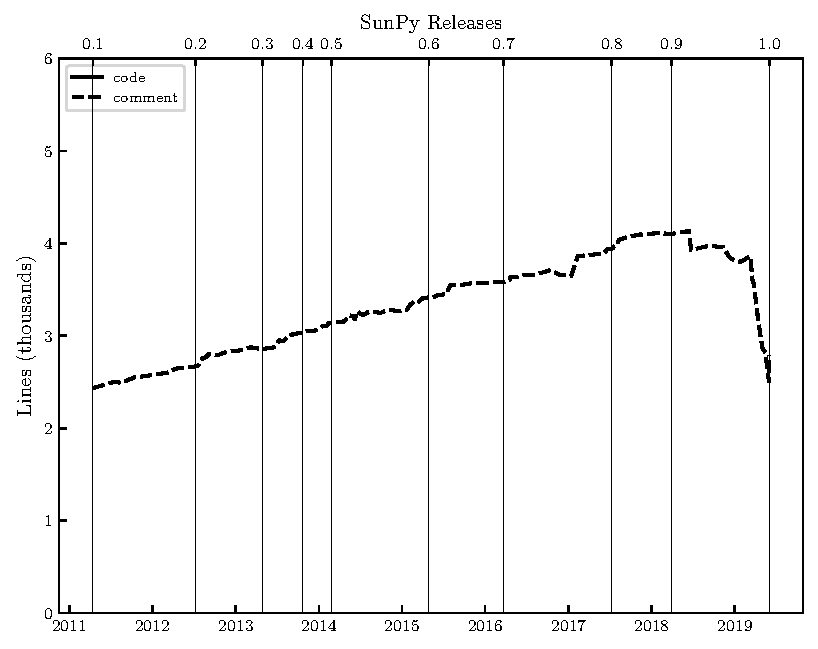
\includegraphics[width=0.5\textwidth]{figures/fig_loc_vs_time.pdf} &
  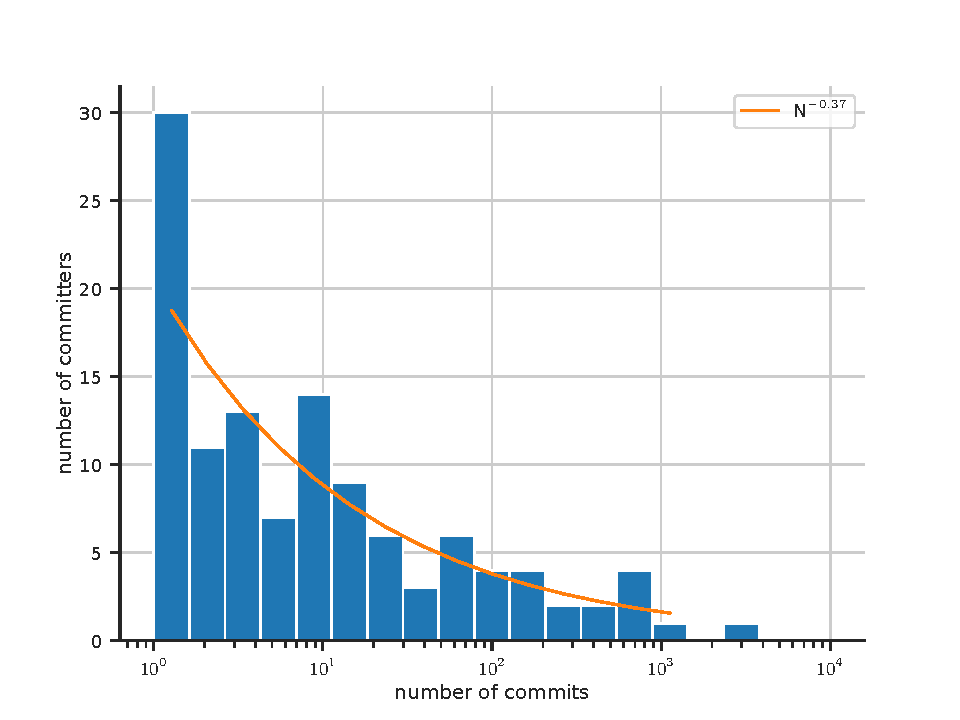
\includegraphics[width=0.5\textwidth]{figures/busfactor_plot.pdf} \\
(a) & (b) \\
\end{tabular}
\begin{tabular}{c}
  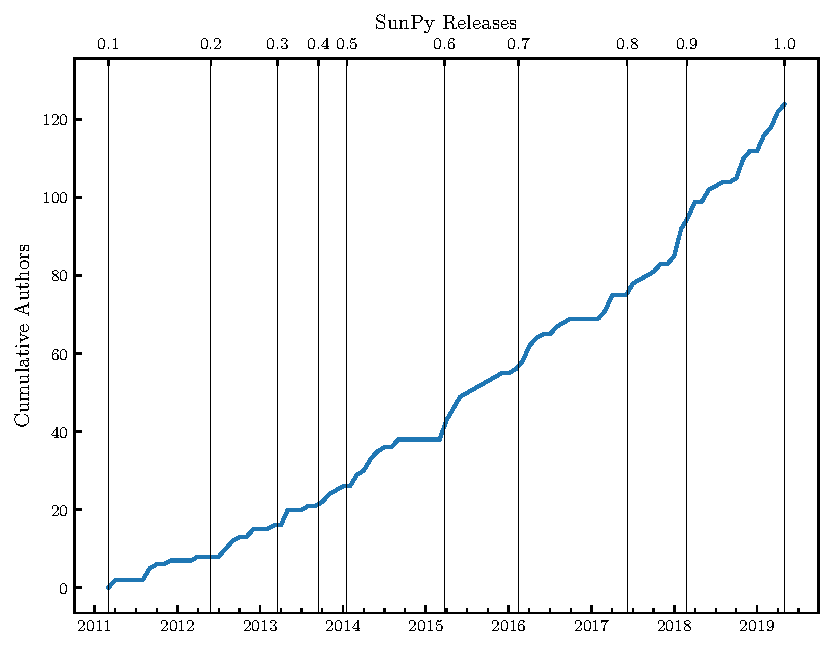
\includegraphics[width=0.5\textwidth]{figures/cumulative_authors.pdf} \\
(c) \\
\end{tabular}
\caption{
	(a) A plot of the the number of lines of code (solid line) and documentation line count (dotted line) as a function of time.
	Major releases are indicated by vertical lines.
	This shows a steady increase of the \sunpypkg codebase with larger additions to our documentation over the last few major versions of \sunpypkg.
	A striking reduction in the code base occurred after version 0.9.
	This period saw a major code organization and deletion of obsolete features along with removing support for Python 2.
	(b) A plot of the number of commits as a function of the number of authors.
	It should be noted that the number of commits is not a 100\% useful measure as any one commit could have as many code or line changes as the previous 100 commits.
	However, it does indicate the majority of commits within the package are undertaken by the least amount of people with an average individual contribution of less than 10 commits.
	(c) This figure charts the cumulative number of authors (i.e., committers) to \sunpypkg as a function of time which shows a steady increase in the number of people involved in the development team.
}
\label{fig:metafig}
\end{figure}
